\bigskip
\begin{center}\textsc{Gauss} an \textsc{Gerling}.\quad Göttingen, 5. Junius 1838.\end{center}

Nach einem Theorem, wovon ich nicht bestimmt weiss, ob ich es Ihnen
früher schon mitgetheilt habe, muss man, wenn in einem Dreieckssystem $p$
Punkte durch $l$ Linien verbunden sind, gleichviel ob die Richtungen der letztern
bloss einseitig oder hin und zurück festgelegt sind, ausser den Bedin-\par
\makeatletter
\def\ps@gaussIXfortyonestar{\def\@oddhead{}\def\@evenhead{}\def\@oddfoot{\hfil41\textsuperscript{*}\hspace{2em}}\let\@evenfoot\@oddfoot}
\makeatother
\thispagestyle{gaussIXfortyonestar}
\clearpage
\noindent324\hfill\textbf{BRIEFWECHSEL.}\par\medskip
\noindent gungsgleichungen der (ersten und) zweiten Klasse [den Horizontabschlüssen
und den Winkelgleichungen] noch $l-2p+3$ von einander unabhängige Bedingungsgleichungen
erhalten. \textls[120]{Weder mehr noch weniger.} Es kann sich
zwar fügen, dass diese nicht alle in die Form der dritten Klasse [der Seitengleichungen]
gebracht werden können, z.\ B.\ bei einem Dreieckskranze.
\begin{center}
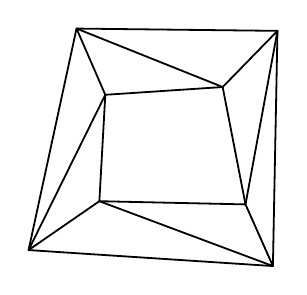
\begin{tikzpicture}[x=.58cm,y=.58cm,line width=.65pt,line cap=round,line join=round]
\coordinate (A) at (1.05,5.3);
\coordinate (B) at (5.45,5.25);
\coordinate (C) at (5.35,0.1);
\coordinate (D) at (0,0.45);
\coordinate (E) at (1.68,3.85);
\coordinate (F) at (4.25,4.02);
\coordinate (G) at (4.75,1.45);
\coordinate (H) at (1.55,1.52);
\draw (A)--(B)--(C)--(D)--cycle;
\draw (E)--(F)--(G)--(H)--cycle;
\draw (A)--(E) (A)--(F) (B)--(F) (B)--(G)
      (C)--(G) (C)--(H) (D)--(H) (D)--(E);
\end{tikzpicture}
\end{center}

Allein ich nehme auf diese Ausnahme keine Rücksicht, da sie bei Ihrem
System unnöthig ist.

Ich zähle nun
\[
\begin{aligned}
p&=24\ \text{Punkte}\\
l&=66,\ \text{nemlich }\begin{aligned}[t]22\ &\text{einseitige Richtungen,}\\44\ &\text{conjugirte Richtungen,}\end{aligned}
\end{aligned}
\]
so dass 21 Bedingungsgleichungen quaestionis da sein müssen, und so viele
haben Sie wirklich. Die Unabhängigkeit kann man prüfen, wenn man die $p$
schicklich ordnet, wobei ich von der Ordnung Ihrer Zahlen 1 .\ .\ .\ .\ 112 zum
Theil habe abgehen müssen, und das nemliche Theorem wiederholt anwendet,
indem man $p$ successive vollständig werden lässt. Auch diese Prüfung haben
Ihre 21 Gleichungen bestanden. In \textls[120]{Ihren} Zahlen ist einige Confusion; 24
und 61 fehlen, so dass zusammen (wie oben $22+2\mathbin{.}44)=110$ Richtungen herauskommen,
und 112 steht am unrechten Platze.

Nach dieser Prüfung zweifle ich nicht, dass Sie Ihre 21 Gleichungen
dreist serviren können.

Habe ich übrigens recht gezählt, so müssen Sie 24 Bedingungsgleichungen
der $2^{\mathrm{ten}}$ Klasse haben.

Nur auf einen Umstand bei der Ausführung muss ich Sie noch aufmerksam
machen. Habe ich es vielleicht schon früher gethan, so entschuldigen
Sie meine Vergessenheit mit der guten Absicht.

Sie weichen in der Aufstellung Ihrer Tableaus darin von meiner Form
ab, dass Sie alle Richtungen von \textls[120]{einer derselben} an zählen, während ich
von einer gewissermaassen willkürlichen, richtiger von einer dem System\par
\clearpage
\noindent\textbf{ZUR NETZAUSGLEICHUNG.}\hfill325\par\medskip
\noindent fremden, an zähle. Sie dürfen daher bei der Ausführung nicht vergessen,
dass sämmtliche Richtungen gleich zuverlässig, oder richtiger, gleich unzuverlässig
sind, und dass Sie also Ihr jedesmaliges 0 mit unter die Correctionsbedürftigen
setzen müssen. Der Erfolg wird übrigens immer der sein, dass
die Summe aller Correctionen an Einem Standpunkt $=0$ wird.

\begingroup
\def\letterfivestars{*}
\makeatletter
\renewcommand{\@makefnmark}{\hbox{\normalfont[\textsuperscript{\letterfivestars})]}}
\renewcommand{\@makefntext}[1]{\parindent1em\noindent\hbox to2.4em{\hss[\textsuperscript{\letterfivestars})\ }#1]}
\makeatother
Ich bewundere aber Ihre Intrepidität, eine so grosse Eliminationsarbeit
zu übernehmen. Ich würde einen gleichen Muth nicht gehabt haben. Bei
meinen 33 Punkten war die Anzahl der Bedingungsgleichungen $3^{\mathrm{ter}}$ Klasse
[der Seitengleichungen] viel kleiner (ich glaube 7)\footnote{Es sind deren 12.}; das Eliminiren, indem
man zuerst nur die der $2^{\mathrm{ten}}$ Klasse [der Winkelgleichungen] berücksichtigt, war
trotz der grossen Zahl auf indirectem Wege leicht und Fehler der Rechnung
unmöglich, und der Umstand, dass sämmtliche Richtungen hin und zurück
gemessen waren, verstattete sehr erleichternde Modificationen und ein schnelles
Hingelangen zu stehenden Resultaten. Ich fürchte, dass letzteres bei Ihnen in
viel geringerm Grade stattfinden wird\def\letterfivestars{**}\footnote{Vergl. S.\ 250/251.}. Wollen Sie aber einmal den Zweck,
so gibt es kein Mittel als Aufmerksamkeit und Geduld.

Hätte ich selbst diese Rechnungen zu führen gehabt, so würde ich die
drei Plätze, wo nicht gemessen ist, gar nicht in das System aufgenommen
haben, nicht weil ich es missbillige, sondern weil ich die grosse Arbeit gescheut
haben würde. Würden alle nur einseitig beobachteten Richtungen ausgeschlossen,
so würde die Compensation des Systems sehr leicht sein, aber
freilich gewinnt bei Ihrer Unternehmung die Sicherheit durch vollständige
Berücksichtigung sehr bedeutend. .\ .\ .\ .\ .\ .

Das Arrangement bei den Vierecken ist übrigens an sich willkürlich,
und nur um die Willkür abzuschneiden, befolge ich die von Ihnen citirte
Regel\def\letterfivestars{***}\footnote{Vergl. den Brief an \textsc{Gerling} vom 11. Februar 1824, S.\ 249. \textsc{Gerling} hatte in Bezug darauf
(am 2. Juni 1838) geschrieben: »Ich habe mir von dem Grunde der Regel bis jetzt keine andere Rechenschaft
geben können, als dass auf diese Weise verhältnissmässig die grössten Coefficienten zum Vorschein
kommen.«}, die weiter keinen Vorzug hat, als den von Ihnen richtig errathenen.
\endgroup
